\begin{figure}[t]
  \centering
  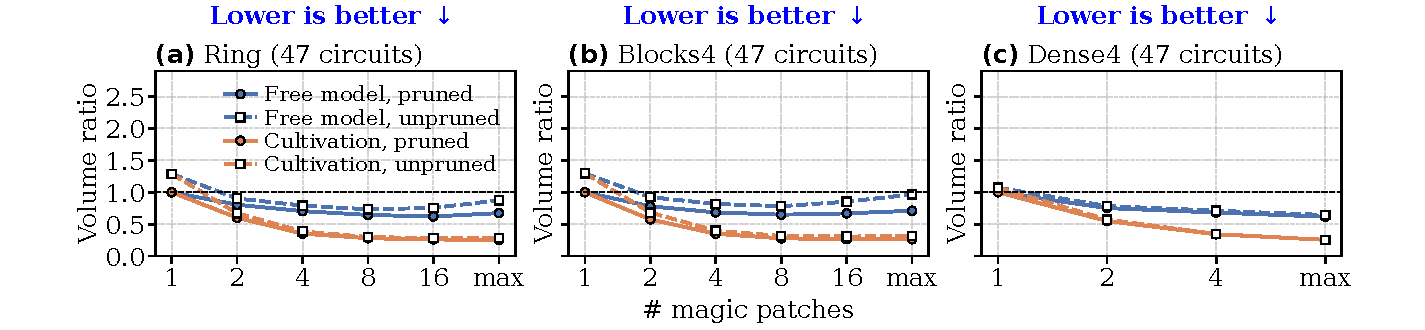
\includegraphics[width=\linewidth]{figures/evaluation/fig_rq3_provisioning.pdf}
  \caption{\textbf{Layout provisioning} (RQ3). Space--time volume as the working layout provides more magic-state patches, relative to the pruned volume with a single magic-state patch, on the \textbf{(a)}~ring, \textbf{(b)}~blocks-of-four, and \textbf{(c)}~dense template. Filled markers show the reported (pruned) volume, open markers the volume of the working layout before pruning. \emph{max} uses every magic-state patch of the template.}
  \label{fig:rq3-provisioning}
\end{figure}
